%!TEX root = index.tex
\chapter[Revisão Bibliográfica]{Revisão Bibliográfica}
\label{chap:revisao}
\section{Parceria Universidade-Empresa}
\label{cha:ensino}
\subsection{A universidade empreendedora}
\label{cha:univ_empreend}

Ao longo da história as universidades sofreram alterações no seu papel diante da visão da sociedade, mudando grande parte de suas características e atividades. Segundo \citeonline{etzkowitz2001}, duas revoluções aconteceram no modelo de funcionamento da universidade.

Como instituições de origem medieval, as universidades tinham como principal objetivo a conservação, preservação e transmissão de sua cultura através das gerações. Conforme o passar dos anos e novas descobertas sendo feitas, surgiram os seminários como principal forma de disseminação de conhecimento, até evoluirem para os modelos de ensino similares aos atuais. Caracteriza-se essa fase anterior às revoluções como centrada no ensino.

A primeira revolução acadêmica ocorre com a evolução dos modelos de ensino e universidades adotando um modelo intenso de pesquisa, com a intenção de promover avanços na ciência. Com a transmissão mais acessível de pequenas novas descobertas, as pesquisas começaram a se basear em outras pesquisas já realizadas, gerando um ambiente de pesquisa colaborativa.  Durante e após a Segunda Guerra Mundial nos Estados Unidos, a estrutura de pesquisas começou a receber grandes aportes financeiros, e a equipe de pesquisas começou a crescer de tal forma que foram surgindo necessidades de responsabilidades além das exercidas por alunos e pesquisadores, principalmente em relação à administração dessa estrutura de pesquisas, como manutenção da propriedade intelectual e divulgação de novas descobertas. O ambiente de pesquisas começou a ficar similar a uma empresa, o que levou a segunda revolução da academia.

Com uma estrutura voltada a acelerar o desenvolvimento de pesquisas, os laboratórios passaram a ser vistos como fonte de resolução de problemas reais do mercado. A segunda revolução acadêmica aconteceu quando as universidades passaram a utilizar seus laboratórios de pesquisa para realizar descobertas que pudessem gerar produtos comerciáveis. Desta forma, também foi inserido o desenvolvimento econômico como uma nova missão da universidade, além da pesquisa e do ensino.

\begin{figure}
\caption{Revoluções Acadêmicas}
\centerline{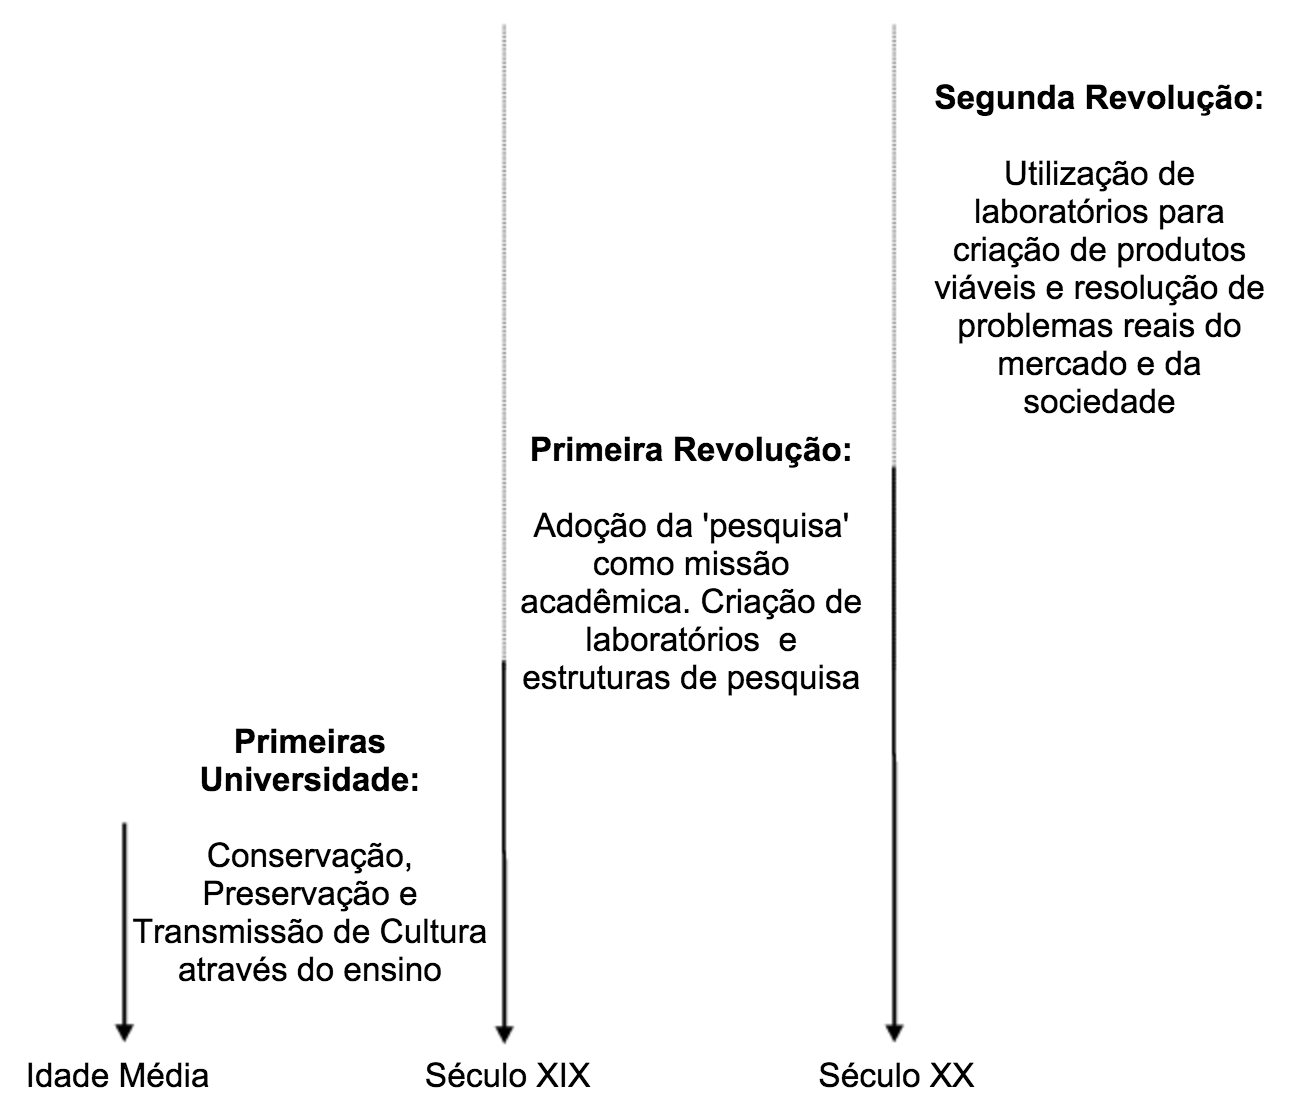
\includegraphics[scale=0.5]{img/academic_revolutions}}
\label{fig:academic_revolutions}
\caption* {Fonte: Elaborado pelo autor a partir de \citeonline{etzkowitz2001}}
\end{figure}

Com o sistema de financiamento de pesquisa da Universidade em  busca de estabilidade, em muitos casos cabe à própria Universidade procurar por novas fontes de receita, gerando novas parcerias com empresas dispostas a investir seu dinheiro em pesquisas.

Dessa forma, surge o conceito de Universidade Empreendedora, que recebe diferentes concepções de diversos autores. Segundo \citeonline{etzkowitz2001}, é uma instituição que trabalha ativamente na transferência de tecnologia e no desenvolvimento econômico, já para \citeonline{burton} é uma instituição que realiza um esforço contínuo de reformulação institucional de forma a melhorar o desempenho para com empresas e o governo, e para \citeonline{plonsky} é uma instituição que exerce um papel ativo no mercado do conhecimento.

\subsection{Interação universidade-empresa-governo}
\label{cha:univ_empreend}

\citeonline{etzkowitz2000} propõe que os modelos de interação entre universidade e empresa refletem na interferência de um terceiro agente, o Governo - ou Estado. Em regimes com forte influência do Estado, como na ex-União Soviética e países do Leste Europeu, o governo regula e direciona as relações entre as empresas e a academia. \ref{fig:triplehelix1}. Esse modelo é visto como um modelo de desenvolvimento falho, pois inibe iniciativas de inovação a partir da empresa e academia, cabendo apenas ao Estado direcionar os estudos a serem realizados.

\begin{figure}[H]
\caption{Modelo de interação universidade-indústria-governo regulado pelo governo}
\centerline{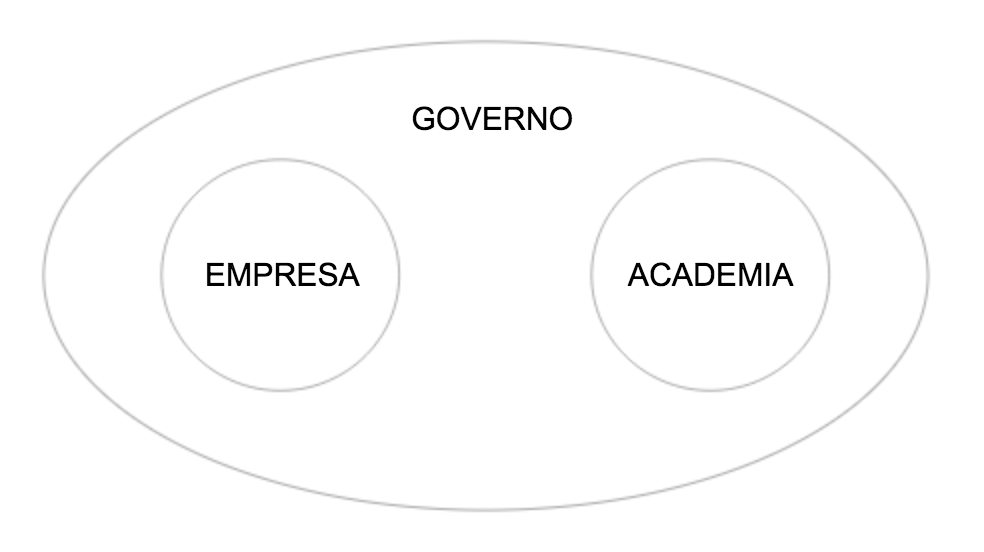
\includegraphics[scale=0.5]{img/triplehelix1}}
\label{fig:triplehelix1}
\caption* {Fonte: Adaptado de \citeonline{etzkowitz2000}}
\end{figure}

Um segundo modelo, apropriado da expressão \textit{laissez-faire}, consiste na minimização da interferência de atuação entre as esferas, principalmente em relação ao Governo, que apresentava total controle no primeiro modelo. Nesse modelo, \ref{fig:triplehelix2}, cada ator atua de forma independente, apenas havendo transmissão de informação entre eles mas não uma colaboração ativa em prol da inovação.

\begin{figure}[H]
\caption{Modelo \textit{laissez faire}, de independência entre universidade, indústria e governo}
\centerline{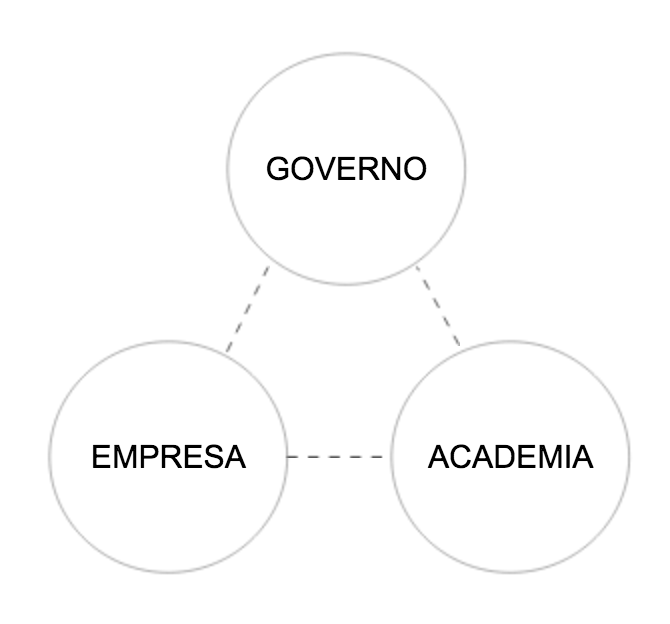
\includegraphics[scale=0.5]{img/triplehelix2}}
\label{fig:triplehelix2}
\caption* {Fonte: Adaptado de \citeonline{etzkowitz2000}}
\end{figure}

Já o terceiro modelo em questão representa de fato a Tripla Hélica Universidade-Indústria-Governo, com uma infraestrutura de conhecimento compartilhada entre as esferas, com funções surgindo através da colaboração, cogestão e compartilhamento de recursos entre os atores, através de organizações emergindo nessas interfaces.


\begin{figure}[H]
\caption{Modelo Tripla Hélice Universidade-Empresa-Governo}
\centerline{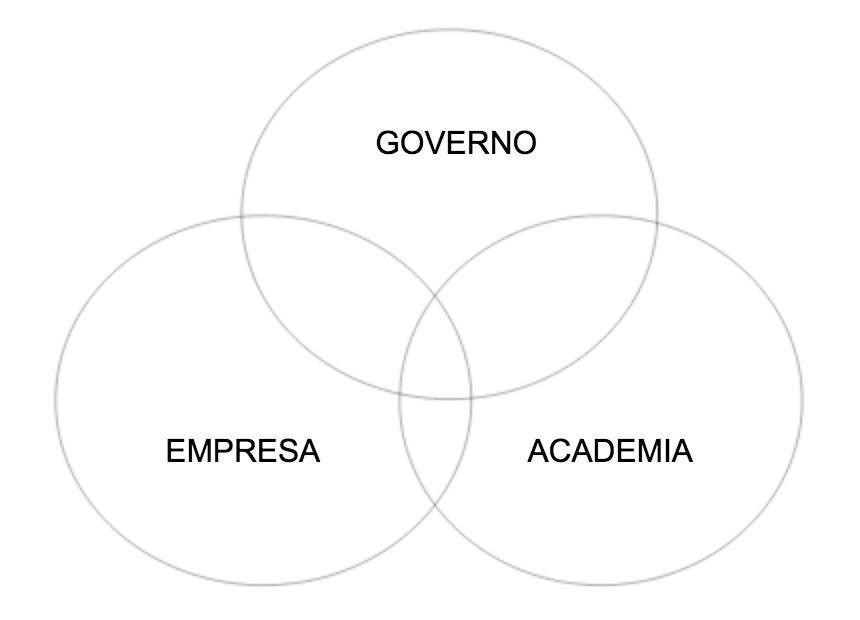
\includegraphics[scale=0.5]{img/triplehelix3}}
\label{fig:triplehelix3}
\caption* {Fonte: Adaptado de \citeonline{etzkowitz2000}}
\end{figure}

No modelo de tripla hélice o Governo assume uma posição de facilitador da interação entre empresa e academia sem tirar a autonomia de ambos os atores. Através de leis de incentivo e financiamento o governo fornece e capta recursos para o desenvolvimento de novas pesquisas, e através da criação de laboratórios e parques tecnológicos oferece uma infraestrutura para  auxiliar no processo de inovação.

\subsection{Desafios da gestão universidade-empresa}
\label{cha:univ_empreend}

\citeonline{plonsky} ressalta a mudança de ênfase da discussão sobre a cooperação entre academia e setor produtivo na época, pois a temática principal deixou de ser ideológica, e sim em relação a gestão dessa parceria. De forma a elucidar essa questão ele define alguns principais desafios gerenciais entre universidade e empresa para manter a relação entre ambos "benéfica e transformadora":

\begin{itemize}
\item Compartilhar uma visão multidimensional e integrada da cooperação universidade-empresa, centrada no desenvolvimento de competências humanas
\item Perceber com clareza as missões distintas, mas complementares, da empresa e da universidade no processo de inovação
\item Desenvolver respostas inovativas às diversas necessidades de cooperação empresa-universidade
\item Capacitar para a gestão eficaz da cooperação empresa-universidade
\end{itemize}

Primeiramente, ambos os lados devem entender que a parceria entre academia e empresa não se limita a projetos específicos e pontuais envolvendo ambas as partes, pois na realidade a parceria se extende a um dos principais objetivos da universidade, que é o de desenvolver alunos para atuar no mercado de trabalho. De forma geral, o setor produtivo deve estar sempre estar interessado na qualidade e na atualização do ensino das universidades pois consequentemente serão formadas pessoas mais capacitadas.

Em seguida, deve ficar evidente que empresa e universidade possuem papéis distintos no processo de inovação. A universidade assume na inovação o papel de organizar todo o conhecimento em relação a determinados assuntos. Já o desenvolvimento de tecnologia corresponde à aplicação do conhecimento organizado na produção de bens e serviços e, de forma geral, é de responsabilidade da empresa.

Embora existam diferentes necessidades de ambas as partes advindas da parceria universidade-empresa, deve-se compreender que por mais que a relação seja assimétrica, uma verdadeira cooperação não só deve ser benéfica como também deve gerar aprendizado para ambas as partes. Logo as respostas inovativas devem surgir mais rapidamente com ambos os lados sendo capacitados e beneficiados.

Por fim, todo caso de cooperação empresa-universidade deve estar sob gestão de um \textit{staff} pré-capacitado, pois uma série de conhecimentos acabam sendo necessários para tirar o máximo de proveito dessa parceria, como: desdobramento de missão e visão institucional; proteção de propriedade intelectual; equacionamento econômico-financeiro, gestão de projetos, entre outros.

\section{\textit{Benchmarking} de parcerias universidade-empresa:} % (fold)
\label{sec:cases}

\subsection{TECNOPUC}

Os parques tecnológicos são um movimento de apoio à inovação e empreendedorismo que têm crescido muito nos últimos anos no Brasil. Eles se referem a aglomerações de empresas de base tecnológica, que podem ser pequenas ou não, articuladas a universidades e centros de P\&D, possibilitando sinergias decorrentes da proximidade entre os atores. \cite{parquestecnologicos} 

No Brasil há varios parques tecnológicos de destaque, como o Porto Digital em Recife, o Parque Tecnológico de São José dos Campos, o Parque Tecnológico da UFRJ e o Parque Científico e Tecnológico da PUC-RS (TECNOPUC). Dentre esse parques, a TECNOPUC se mostra um excelente caso de sucesso entre universidade e empresa, estimulando a pesquisa e a inovação por meio de uma ação simultânea entre academia, instituições privadas e governo, sob gestão da própria universidade.

O TECNOPUC possui um portfólio de empresas multissetorial, focado em quatro principais áreas definidas a partir da competência acadêmica da Universidade, envolvendo grupos de pesquisa científica e tecnológica, cursos de pós-graduação e à existência de demanda da sociedade. (Figura \ref{fig:tecnopuc})

\begin{figure}
\caption{Áreas de atuação do Tecnopuc}
\centerline{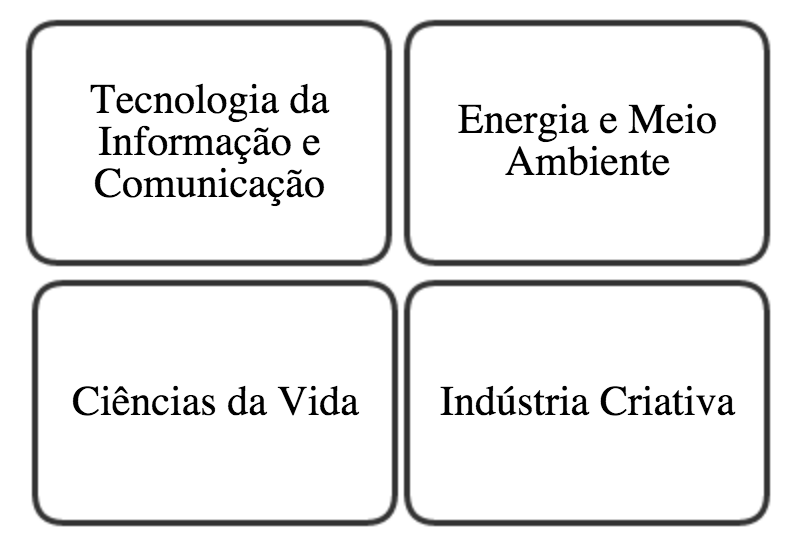
\includegraphics[scale=0.5]{img/tecnopuc}}
\label{fig:tecnopuc}
\caption* {Fonte: Adaptado do site do Tecnopuc}
\end{figure}

Atualmente, o TECNOPUC abriga 120 organizações, desde grandes companias de tecnologia como Samsung, Microsoft, Motorola e Dell até instituições financeiras como o HSBC. 

O TECNOPUC é um dos pilares do INOVAPUCRS - Rede de Inovação e Empreendedorismo da PUC-RS. Segundo \citeonline{tecnopuc}, o sucesso da iniciativa de inovação e empreendedorismo na universidade se deve à combinação do TECNOPUC com diversas outras estruturas de apoio:

\begin{description}
\item[AGT] - A Agência de Gestão Tecnológica facilita e articula a comunicação entre empresa e pesquisadores, identificando possíveis parcerias, acelerando a burocracia inerente a essas parcerias e captando recursos para viabilizar os projetos
\item[ETT] - O Escritório de Transferência de Tecnologia é responsável pelo estabelecimento e proteção das diretrizes de propriedade intelectual das pesquisas geradas em parcerias com empresas.
\item[IDEIA] - O Instituto de Pesquisa e Desenvolvimento possui uma infraestutura laboratorial para incubar projetos de diversas unidades acadêmicas.
\item[RAIAR] - A Incubadora Raiar é responsável por abrigar empresas derivadas de pesquisas estabelecidas na universidade por alunos, professores ou funcionários ou novos empreendimentos de empresas já estabelecidas no TECNOPUC.
\item[LABELO] - Os Laboratórios Especializados em Eletroeletrônica trabalha na prestação de serviços tecnológicos, apoiando o fortalecimento e a qualificação dos produtos para atender a regulamentos e normas internacionais.
\item[CI] - O Centro de Inovação é uma parceria feita com a Microsoft de forma a acelerar o uso de novas tecnologias e fomentar a indústria de software.
\item[NE] - O núcleo empreendedor tem como objetivo estimular o empreendedorismo na Universidade através de palestras, eventos e projetos que visam as oportunidades de mercado e a inovação.
\end{description}

O TECNOPUC tem como missão criar uma comunidade de pesquisa e inovação transdisciplinar por meio da colaboração entre academia, empresas e governo visando aumentar a competitividade dos seus atores e melhorar a qualidade de vida de suas comunidades. Ele se baseia nos seguintes objetivos:

\begin{itemize}
\item Atrair empresas de pesquisa e desenvolvimento (P,D e I) para trabalhar em parceria com a Universidade
\item Promover a criação e o desenvolvimento de novas empresas de base tecnológica
\item Atrair projetos de pesquisa e desenvolvimento tecnológico em geral
\item Estimular a inovação e a interação empresas-Universidade
\item Gerar uma sinergia positiva entre o meio acadêmico e o empresarial
\item Atuar de forma coordenada com as esferas governamentais, particularmente no âmbito do Projeto Porto Alegre Tecnópole
\end{itemize}

\subsection{Porto Digital}

// PARAFRASEAR PORTO DIGITAL

O Porto Digital é um dos principais parques tecnológicos e ambientes de inovação do Brasil e é um dos representantes da nova economia do Estado de Pernambuco. Localizado no Recife, sua atuação se dá nos eixos de software e serviços de Tecnologia da Informação e Comunicação (TIC) e Economia Criativa (EC), com ênfase nos segmentos de games, multimídia, cine-vídeo-animação, música, fotografia e design.

Reconhecido por sua territorialidade singular entre parques tecnológicos, o Porto Digital é um parque urbano instalado no centro histórico do Bairro do Recife e no bairro de Santo Amaro, totalizando uma área de 149 hectares. A região, antes degradada e de pouca importância para a economia local, vem sendo requalificada de forma acelerada em termos urbanísticos, imobiliários e de recuperação do patrimônio histórico edificado desde a fundação do parque, em 2000. Desde a fundação do Porto Digital, já foram mais de 50 mil metros quadrados de imóveis históricos restaurados em toda a extensão territorial do parque tecnológico.

O Porto Digital é fruto e referência nacional de uma ação coordenada entre governo, academia e empresas, conhecido como modelo "Triple Helix". Essa iniciativa propiciou o ambiente necessário para fazer com que o Porto Digital se transformasse num dos principais ambientes de inovação do País. 

Atualmente, o Porto Digital abriga 250 empresas, organizações de fomento e órgãos de Governo e cerca de 7.100 trabalhadores. Desde o final de 2014, o parque também opera nas cidades de Caruaru e Petrolina, localizadas respectivamente no Agreste e Sertão do Estado. O Porto Digital foi considerado pela Associação Nacional de Promotoras de Empreendimentos Inovadores (Anprotec), em 2007 e 2011, o melhor parque tecnológico do Brasil. Em 2005 o ambiente foi considerado o maior do País pela A.T. Kearney.



\subsection{\textit{Deutsche Telekom - T-labs}}

A \textit{Deutsche Telekom} (DT) é uma empresa de telecomuniçação Alemã e também a maior do setor em toda a União Européia. A compania possui um grande expertise na área de tecnologia da comunicação e tecnologia da informação, possuindo duas grandes subsidiárias: a operadora T-mobile e a consultoria de TI T-Systems, ambas com atuação global.

Por atuar em um segmento tão competitivo e totalmente dependente de inovações tecnológicas para gerar vantagem competitiva diante das outras empresas, a DT sempre apresentou muitas iniciativas e um forte investimento na área de P\&D. Através de uma dessas iniciativas surgiu a proposta dos Laboratórios \textit{Deutsche Telekom} (T-labs).

Os T-labs foram criados com o objetivo de pesquisar e desenvolver Tecnologia da Informação e Tecnologia da Comunicação de forma a permitir que novos negócios surjam e que operações já existentes sejam expandidas e acelerar o processo de inovação através da colaboração indústria e academia. \cite{dtlabs}

Para validar a real necessidade da DT em criar os laboratórios, foram levantadas as motivações apresentadas na tabela \ref{tab:motivacoes_dt}

\begin{table}[h]
\begin{center}
\caption{Fontes de Motivação para fundação dos T - Labs}
\label{tab:motivacoes_dt}
\begin{tabular}{>{\raggedright}p{0.25\linewidth}>{\raggedright\arraybackslash}p{0.55\linewidth}}
	\hline
    Importância & Indústria \\ 
    \hline \\
    \multirow{2}{*}{Razão Principal} 
    & Acesso à Inovação \\
    & Obter na fonte últimos avanços tecnológicos \\ \\
	\multirow{2}{*}{Alta relevância}
	& Constante atualização do \textit{know-how} \\
	& Canal de Recrutamento \\ \\
	\multirow{2}{*}{Média importância}
	& Diminuição de risco com pesquisas \\
	& Estabelecer projetos de longo prazo \\ \\
	\multirow{2}{*}{Baixa importância}
	& Diminuição de custos \\
	& Uso de laboratório \\ \\
\end{tabular}%
\caption* {Fonte: \citeonline{dtlabs}}
\end{center}
\end{table}

De forma geral, a DT buscava nos laboratórios uma porta de entrada para descobertas e inovações tecnológicas, além de possíveis novos funcionários e pesquisas de longo prazo.

Dadas as necessidades listadas, a DT sabia que o próximo passo para viabilizar o laboratório seria ultrapassar algumas barreiras existentes em parcerias universidade-empresa: barreiras culturais, institucionais e operacionais. \cite{barriers}

Em relação às barreiras culturais, foram definidos três principais pontos:
\begin{itemize}
\item Apenas são empregados pós doutorados com interesse em pesquisa orientada pela aplicação dos resultados da pesquisa
\item Políticas de publicação e de direito à propriedade intelectual foram bem definidas, com prazos e condições bem descritos
\item Compartilhamento de espaço físico e políticas internas tanto para o \textit{staff} acadêmico quanto da indústria.
\end{itemize}

Em relação às barreiras institucionais:
\begin{itemize}
\item Divisão de objetivos bem definida, com o \textit{staff} da academia voltado para a pesquisa estratégica, e o \textit{staff} da indústria voltado para atividades orientadas pelo desenvolvimento e inovação.
\item Resultados esperados pré definidos através de KPIs, de tal forma que cada área já sabe o que é esperado de si.
\item Separação e autonomia da gestão do laboratório por parte da empresa, de tal forma que mudanças corporativas na DT pouco interfiram no trabalho do laboratório.
\end{itemize}

Em relação às barreiras operacionais:
\begin{itemize}
\item Processos bem definidos 
\item Alinhamento entre áreas feito através da revisão trimestral de projetos e apresentações de progresso
\item Redução do princípio Não-Inventado-Aqui (NIA), no qual as corporações se recusam a usar soluções de terceiros para usar soluções desenvolvidas internamente.
\end{itemize}

